\subsection{Zr($10\bar{1}0$) surface.}
\begin{frame}[t]
\frametitle{Zr($10\bar{1}0$) surface, Oxygen and Hydrogen Absorption}

\small
  This project is carried on in collaboration with Fernando Soto, a Postdoc at 
  Perla Balbuena's group in Texas A\&M University, USA.
  \par
  \vspace{0.5cm}
  Progress so far
  \begin{itemize}
      \item<1-> Oxygen Coverage with alloy elements
	\begin{columns}[c]
	  \column{0.3\textwidth}
	  \centering
	  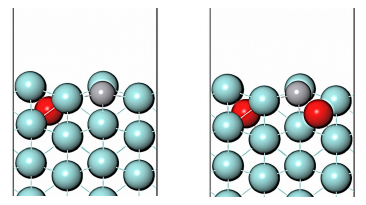
\includegraphics[width=\textwidth]
	  {/home/mariano/CuadernoTrabajo/CV/SLI/02-CurrentResearch/coverage.png}<1>
	  \par
	  \column{0.7\textwidth}
	  \centering
	  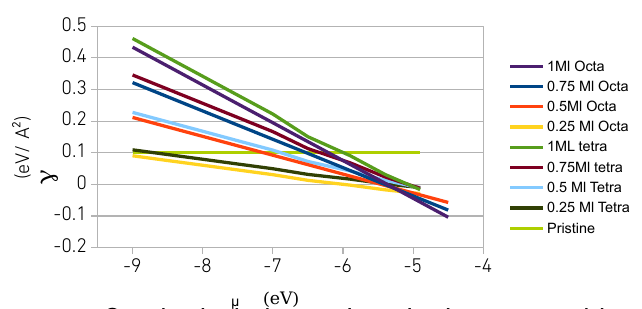
\includegraphics[width=0.7\textwidth]
	  {/home/mariano/CuadernoTrabajo/CV/SLI/02-CurrentResearch/SurfaceEnergies.png}<1>
	  \par
	\end{columns}
      \item<2> AIMD: Hydgrogen moves differently in the presence of Ta and V,

	\begin{columns}
	  \column{0.6\textwidth}
	  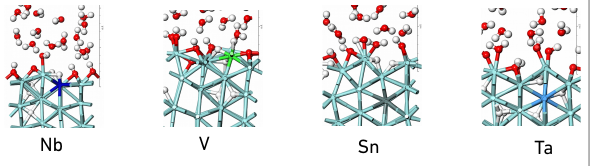
\includegraphics[width=\textwidth]
	  {/home/mariano/CuadernoTrabajo/CV/SLI/02-CurrentResearch/Alloys-AIMD.png}<2>
	  \column{0.4\textwidth}
	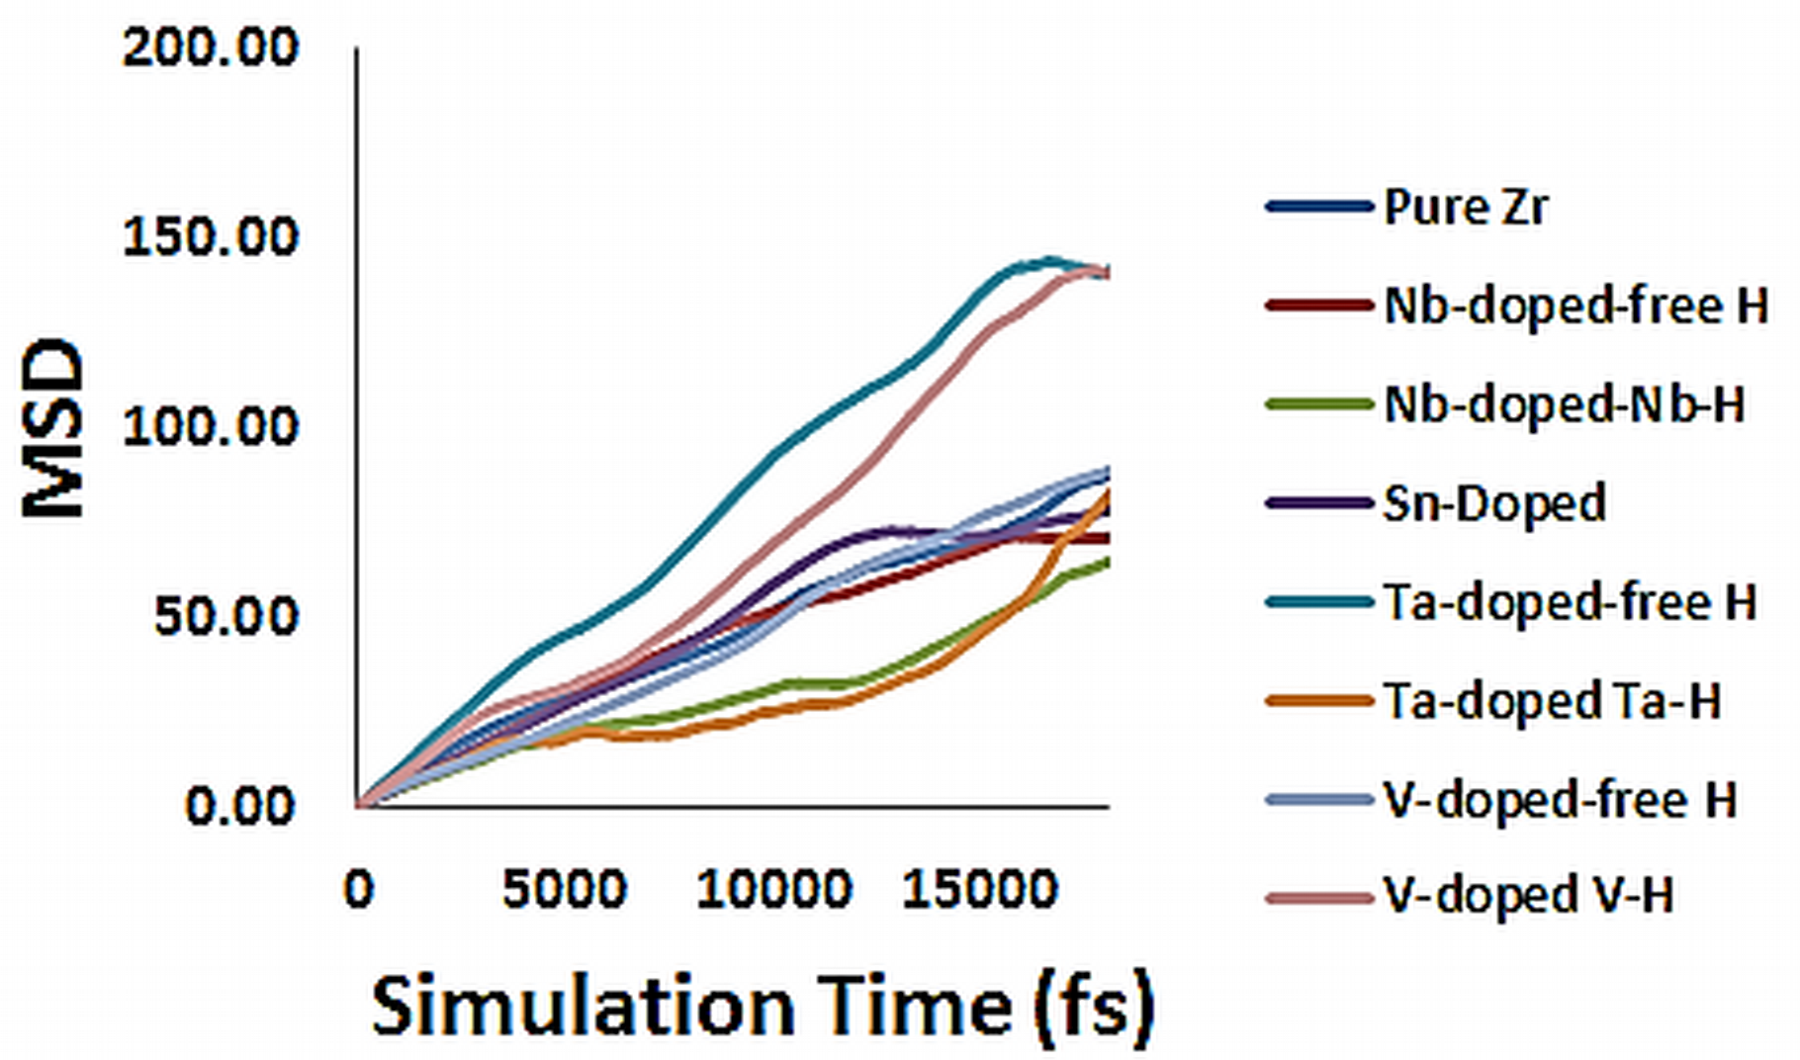
\includegraphics[width=\textwidth]{./02-CurrentResearch/HydrogenMeanFreePaths.png}<2>
	\end{columns}
  \end{itemize}

\end{frame}
